\documentclass[a4paper,11pt,notitlepage]{report}
\usepackage{graphicx}
\usepackage[utf8]{inputenc}
\usepackage[T1]{fontenc}
\usepackage[ngerman]{babel}
\usepackage{bibgerm}
\usepackage{amsmath,amssymb,amsthm}
\usepackage{color}
\usepackage{enumerate}
\usepackage{tabularx}
\usepackage{subfig}
\usepackage{fancyhdr}
\usepackage{upgreek}
\usepackage[pdftex,pdfpagelabels,colorlinks,backref,pagebackref]{hyperref}
\usepackage{tikz} % SELBST HINZUGEFÜGT
\usepackage{graphicx}
\usepackage{framed}
\usepackage{lmodern}
\usepackage{geometry}
\geometry{a4paper,left=20mm,right=30mm, top=3cm, bottom=2cm} 
\usepackage{marginnote}
\setlength{\headwidth}{15cm}
\setlength{\textwidth}{15cm}

\usepackage{shadethm}
% == Set the heading style ===================================================
\setlength{\headheight}{14pt}
\pagestyle{fancyplain}
\renewcommand{\chaptermark}[1]{\markboth{#1}{}}
\renewcommand{\sectionmark}[1]{\markright{\thesection\ #1}}
\lhead[\fancyplain{}{\thepage}]{\fancyplain{}{\rightmark}}
\rhead[\fancyplain{}{\leftmark}]{\fancyplain{}{\thepage}}
\cfoot{}
\renewcommand{\headrulewidth}{0.4pt}
% ============================================================================

% == Set correct values for fitting floats ===================================
\tolerance=2000
\emergencystretch=10pt

\setcounter{topnumber}{3}
\setcounter{totalnumber}{5}
\setcounter{bottomnumber}{2}

% To make those darn floats fit where they should
\setcounter{totalnumber}{9}
\setcounter{topnumber}{9}
\setcounter{bottomnumber}{9}
\renewcommand{\textfraction}{0.00}
\renewcommand{\topfraction}{1.0}
\renewcommand{\bottomfraction}{1.0}
% ============================================================================

% == German definitions for theorems etc. ==================================== 
%\newtheorem{theorem}{Satz}[chapter]
\newtheorem{lemma}{Lemma}[chapter]
\newtheorem{proposition}{Proposition}[chapter]
%\newtheorem{corollary}{Korollar}[chapter]
\newtheorem{observation}{Beobachtung}[chapter]
\newtheorem{fact}{Fakt}[chapter]
%\theoremstyle{remark} 
\theoremstyle{definition} 
\newtheorem{remark}{Bemerkung}[chapter]
\newtheorem{example}{Beispiel}[chapter]
% ============================================================================

% == Abkürzungen für die reellen, natürlichen, ganzen,... Zahlen =============
\newcommand{\R}{{\ensuremath{\mathbb{R}}}}
\newcommand{\N}{{\ensuremath{\mathbb{N}}}}
\newcommand{\Z}{{\ensuremath{\mathbb{Z}}}}
\newcommand{\C}{{\ensuremath{\mathbb{C}}}}
\newcommand{\Q}{{\ensuremath{\mathbb{Q}}}}
\newcommand{\F}{{\ensuremath{\mathbb{F}}}}
\newcommand{\Prim}{{\ensuremath{\mathbb{P}}}}
% ============================================================================

\newcommand{\RM}[1]{\MakeUppercase{\romannumeral #1{}}} 

% == Makros für Autorenname und -adresse =====================================
\newcommand{\myaddress}[6]{%
  \parbox{\textwidth}{\textbf{\large #1}\\
    #2\\ #3\\ #4\\ 
    \ifthenelse{\equal{#5}{}}{}{Email: \href{mailto:#5}{\texttt{#5}}\\}
    \ifthenelse{\equal{#6}{}}{}{WWW: \href{#6}{\path|#6|}\\}
  } 
}

\newcommand{\myauthor}[1]{%
  \addtocontents{toc}{\protect\hspace{3.35ex}%
  \textsl{#1}\par}\vspace{-4ex}\quad\hfill\textsl{\Large #1}\vspace{8ex}}

\newcommand{\myname}[1]{\Large #1}

%%%%%%%%%%%%%%%%%%%%%%%%%%%%%%%%%%%%%%%%%%%%%%%%%%
% Tragen Sie in der folg. Zeile Ihren Namen ein: %
%%%%%%%%%%%%%%%%%%%%%%%%%%%%%%%%%%%%%%%%%%%%%%%%%%

\newcommand{\OO}{{\ensuremath{\mathcal{O}}}}
\newcommand{\hateq}{{\ensuremath{\stackrel{\wedge}{=}}}}

%\renewcommand{\thechapter}{\Roman{chapter}}
\renewcommand{\thesection}{\arabic{section}}


\newenvironment{Kasten}[1]
{
\hspace{0.05\linewidth}
\begin{center}
\begin{minipage}{0.95\linewidth}
\setlength{\fboxsep}{10pt}
%\setlength{\fboxsep}{18pt}
%\definecolor{shadecolor}{gray}{0.9}
\definecolor{shadecolor}{rgb}{0.9,1,1}
\definecolor{framecolor}{gray}{0}
%\def\FrameCommand{\fcolorbox{framecolor}{shadecolor}}
%\MakeFramed {\FrameRestore}
\subsection*{#1}
%\begin{itshape}
}
{
%\end{itshape}
%\endMakeFramed
\end{minipage}
\end{center}
%\vspace{1em}
}


\newenvironment{bsp}[1]
{
\setlength{\fboxsep}{10pt}
\subsection*{Beispiel: #1}
\begin{upshape}
}
{
\end{upshape}
}

\newshadetheorem{theorem}{Satz}[chapter]
\newshadetheorem{corollary}{Korollar}[chapter]
\newshadetheorem{definitions}{Definition}[chapter]

\newenvironment{definition}[1]{
	\begin{definitions}
	\marginnote{\emph{#1}}
}{\end{definitions}}

\begin{document}
\shorthandoff{"}
\setcounter{chapter}{0}

\begin{titlepage}
	\begin{center}	
		\LARGE \textbf{{Funktionentheorie - Mitschrieb -} \\[5ex] 
    		{\Large Vorlesung im Sommersemester 2012\\[5ex]}}
	\end{center}
	\begin{center}
		\Large Sarah Lutteropp, Simon Bischof
	\end{center}
	\begin{center}
		\href{mailto:sarah.lutteropp@student.kit.edu}{sarah.lutteropp@student.kit.edu}, 
		\href{mailto:simon-bischof@t-online.de}{simon-bischof@t-online.de}
	\end{center}
	\begin{center}
		\today
	\end{center}
	\vspace{2cm}
	\begin{center}
		%\includegraphics[width=0.8\textwidth]{torus2.pdf}
	\end{center}
\end{titlepage}
%\maketitle
\setcounter{tocdepth}{1}
\tableofcontents

\section*{Zusammenfassung}
Dies ist ein Mitschrieb der Vorlesung “Funktionentheorie” vom Sommersemester 2012 am Karlsruher Institut für Technologie, die von Herrn Dr. Andreas Müller-Rettkowski gehalten wird.

\setcounter{chapter}{-1}
\chapter{Organisatorisches}
\setcounter{section}{-1}

Ausweichtermin Fr. 11:30 Uhr\\
Übungsblatt Dienstags auf Homepage\\
Übungsbetrieb auf Englisch

\section{Themen der Vorlesung}
Ziel der VL: Cauchy Integralsatz\\
$\C$, topologische Grundlage, $f \colon \C \rightarrow \C$ \\
Zweite Hälfte der VL: Anwendungen: Residuensatz

\chapter{Komplexe Zahlen}

\section{Definition der komplexen Zahlen}

\begin{definition}{Definition von $\C$}
Eine komplexe Zahl ist ein geordnetes Paar von rellen Zahlen $(x,y)$

Für $z=(x,y), w=(u,v)$ gilt $(z=w) :\Leftrightarrow x = u$ und $y = v$.
\end{definition}

\paragraph{Exkurs:} Gleichheit bei rationalen Zahlen als Tupel ganzer Zahlen \newline
Hier ist $(1,2)=(2,4)$, denn $(1,2)\hateq \frac{1}{2} = \frac{2}{4} \hateq(2,4)$.


\begin{definition}{Addition und Multiplikation komplexer Zahlen}
	Seien $z = (x,y), w = (u,v) \in \C$.
	$$z+w := (x+u, y+v)$$
	$$z \cdot w := (xu-yv, yu+xv)$$
\end{definition}

\paragraph{Exkurs}
Warum nicht $z \cdot w = (xu, yv)$? \\
$zw = 0 \Leftrightarrow z = 0 $ oder $w=0$ ist falsch!

\begin{theorem}
	Mit $+,\cdot$ wird $\C$ ein Körper.
	\begin{itemize}
		\item $0 := (0,0)$ ist das neutrale Element für $+$
		\item $1 := (1,0)$ ist das neutrale Element für $\cdot$
		\item Inverses zu $z=(x,y)$ bzgl. $+$: $-z := (-x,-y)$
		\item Inverses zu $z=(x,y)$ bzgl. $\cdot$ für $z \neq 0 \Leftrightarrow (x,y) \neq (0,0)$ $\Leftrightarrow x^2 + y^2 > 0: $
		$$\frac{1}{z} = \left(\frac{x}{x^2+y^2}, \frac{-y}{x^2 + y^2}\right)$$
	\end{itemize}
\end{theorem}

\paragraph{Exkurs}
Durch die Körperaxiome folgt:
\begin{itemize}
	\item $z+a=b$ ist (eindeutig) lösbar.
	\item $az = b$ ist (eindeutig) lösbar für $a \neq 0$. 
\end{itemize}

\begin{theorem}
	Seien $x,y \in \R$. Dann gelten:
	\begin{itemize}
		\item $(x,0) + (y,0) = (x+y,0)$
		\item $(x,0) \cdot (y,0) = (xy,0)$
	\end{itemize}
	
	Komplexe Zahlen der Form $(x,0)$ haben dieselben arithmetischen Eigenschaften wie die reellen Zahlen $x$. Deshalb werden die komplexen Zahlen $(x,0)$ mit den reellen Zahlen $x$ identifiziert. Ab jetzt schreiben wir $(x,0) = x \quad \forall x \in \R$.
	
	$$(x,y) = (x,0) + (0,y) = x + (0,1) (y,0) = x + (0,1) y$$
\end{theorem}

\begin{definition}{Imaginäre Einheit}
	$(0,1) =: i$
\end{definition}

\begin{theorem}
	$i^2 = -1$
\end{theorem}

\begin{theorem}
	Für reelle Zahlen $x,y$ hat man $(x,y) = x+iy \quad (=z)$
\end{theorem}

\paragraph{Bemerkung} $x,y$ stehen standardmäßig für reelle, $z$ für komplexe Zahlen.

\section{Rechnen mit komplexen Zahlen}

\begin{definition}{konjugiert komplexe}
	Zu $z = x+iy$ ist $\bar{z} = x - iy$ die konjugiert komplexe Zahl.
	$$x = Re(z), \quad y = Im(z)$$
	Beachte $Im(z) \in \R$!
	\begin{center}
		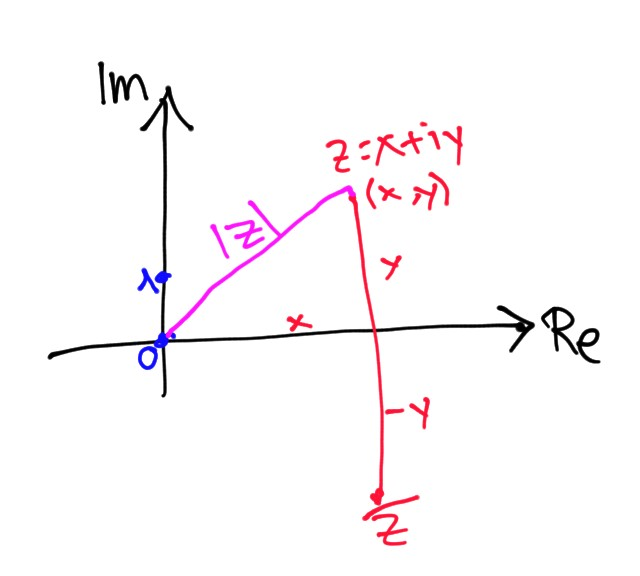
\includegraphics[scale=0.3]{images/16_04_12_01.jpg}
	\end{center}
	Es gelten ($z,w \in \C$): 
	\begin{itemize}
	\item $Re(z+w) = Re(z) + Re(w)$
	\item $Im(z+w) = Im(z) + Im(w)$
	\item Für $z=x+iy$: $x = Re(z) = \frac{1}{2} (z + \bar{z}), Im(z) = \frac{1}{2i} (z - \bar{z}) = y$
	\end{itemize}
\end{definition}

\begin{theorem}
	Seien $z,w \in \C$
	\begin{enumerate}[a)]
	\item $z \in \R \Leftrightarrow z = \bar{z}$
	\item $\bar{\bar{z}} = z$
	\item $\overline{z+w} = \bar{z} + \bar{w}, \overline{zw} = \bar{z} \bar{w}$
	\item $z\bar{z} \in \R, z \bar{z} > 0 \Leftrightarrow z \neq 0, z \bar{z} = 0 \Leftrightarrow z = 0$
	\end{enumerate}
	Zu $d)$: $z = x+iy, z \bar{z} = x^2 + y^2 = |z|^2$
\end{theorem}
	
\begin{definition}{Betrag}
Für $z \in \C$ ist $|z| := \sqrt{z \bar{z}}$ der Betrag.

Speziell: $z = x \in \R: |z| = |x| = \sqrt{x^2}$
\end{definition}

\paragraph{Exkurs}
Beweis von $\overline{(\frac{z}{w})} = \frac{\bar{z}}{\bar{w}}$:

$$\overline{\left(\frac{1}{w}\right)} = \overline{\left(\frac{1 \bar{w}}{w \bar{w}}\right)} = \overline{\left(\frac{\bar{w}}{|w|^2}\right)} = \frac{w}{|w|^2} = \frac{1}{\bar{w}}$$ und dann Verwendung von $\overline{\left(\frac{z}{w}\right)} = \overline{\left(z \frac{1}{w}\right)}$

\begin{theorem}
	$z,w \in \C$.
	\begin{enumerate}[a)]
		\item \textcolor{blue}{$|z| \geq 0$ und $|z|= 0 \Leftrightarrow z = 0$}
		\item $|\bar{z}| = |z|$
		\item $|zw| = |z||w| \Rightarrow |\frac{z}{w}|= \frac{|z|}{|w|}$
		\item $|Re(z)| \leq |z|, |Im(z)| \leq |z|$
		\item \textcolor{blue}{$|z+w| \leq |z| + |w|$}
		\item $|z+w|^2 = |z|^2 + |w|^2 + 2 Re (\bar{z} w)$
		\item $|z-w|$ ist der Abstand von $z$ zu $w$.
		\item \textcolor{blue}{$|\lambda z| = |\lambda| |z|, \lambda \in \R$}
	\end{enumerate}
	\textcolor{blue}{normierter Raum}
\end{theorem}

\begin{proof}
	zu e) $z + w = 0 \checkmark$
	Sei $z+w \neq 0.$
	$1 = Re \frac{z}{z+w} + Re \frac{w}{z+w} \leq \frac{|z|}{|z+w|} + \frac{|w|}{|z+w|}$ \newline Übung: Wann gilt "="?
\end{proof}

\paragraph{Exkurs}
$w = u+iv$\\
$z = x+iy$\\
$z-w = (x-u) + i(y-v)$\\
$|z-w| = \sqrt{(x-u)^2 + (y-v)^2}$

\begin{center}
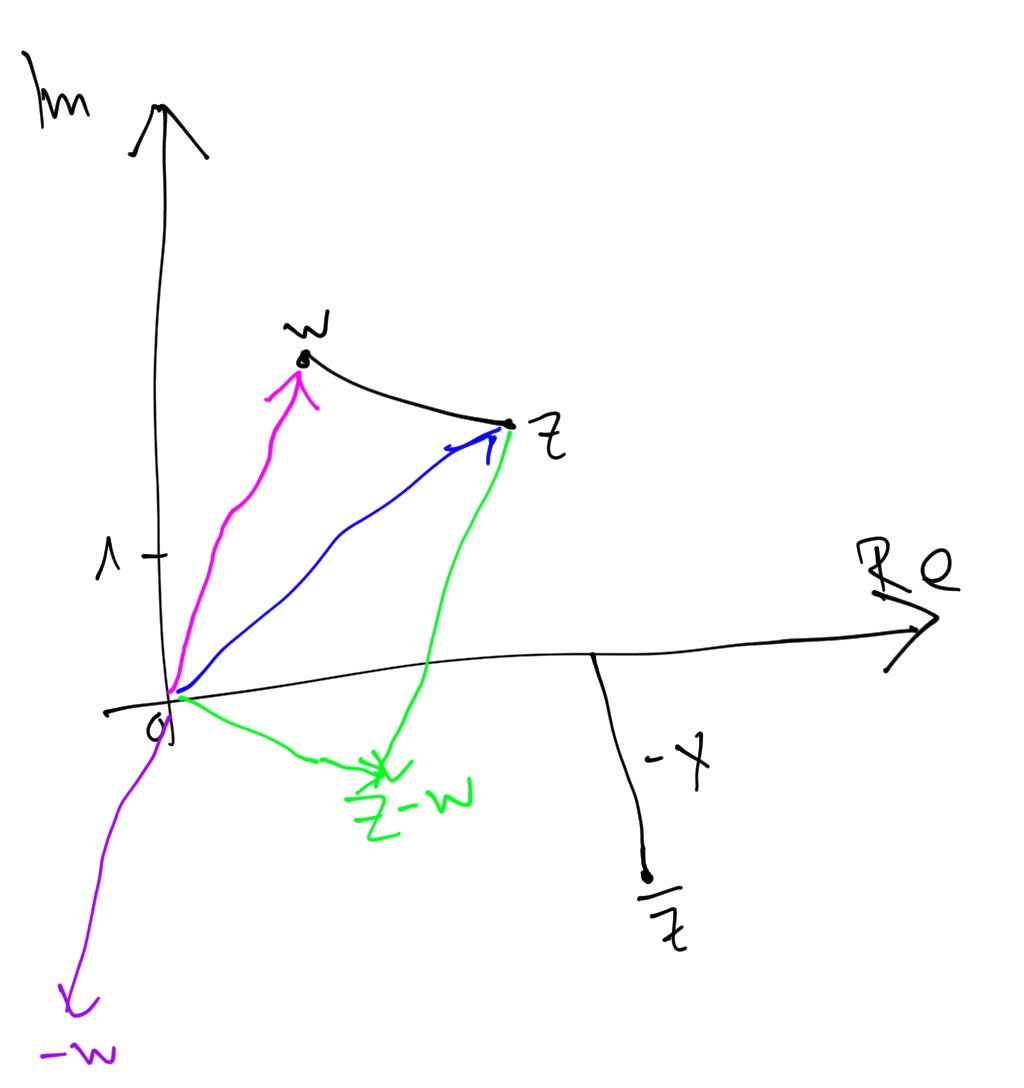
\includegraphics[scale=0.2]{images/16_04_12_02.jpg}
\end{center}

\paragraph{Beispiel}
$\{z \mid |z-5| < 3\}$ ist Kreis um 5 mit Radius 3.

\section{Konvergenz von Folgen komplexer Zahlen}

Durch $d(z,w):= |z-w|, z,w \in \C$ wird auf $\C$ eine \underline{Metrik} definiert.

\begin{definition}{}
$(z_k)$ sei Folge komplexer Zahlen.\newline
$(z_k)$ heißt \underline{konvergent}, falls ein $a \in \C$ existiert mit
$$\lim_{k\to\infty}|z_k-a|=0 \quad \left(\lim_{k\to\infty}z_k=a \text{ oder } z_k\to a (k\to\infty)\right)$$
$$\Leftrightarrow\quad\forall \epsilon>0 \quad\exists n\in\N \quad\forall k\geq n:|z_k-a|<\epsilon$$
$a$ heißt Grenzwert.
\end{definition}

\begin{theorem}{}
$z_k\to a \quad (k\to \infty) \Leftrightarrow
Re(z_k)\to Re(a) \text{ \underline{und} }Im(z_k)\to Im(a) \quad (k\to\infty)$\newline
Denn: $|z_k|^2=(Re(z_k)-Re(a))^2+(Im(z_k)-Im(a))^2$
\end{theorem}

\begin{definition}{Cauchy-Folge}
Die Folge $(z_k)$ heißt \underline{Cauchy-Folge}, falls
$$\forall\epsilon>0 \quad \exists N\in\N \quad \forall k,l\geq N: \quad |z_k-z_l|<\epsilon$$
$\Rightarrow$ Jede konvergente Folge ist eine Cauchy-Folge.
\end{definition}

\begin{definition}{Beschränktheit von Folgen}
Die Folge $(z_k)\subset\C$ heißt \underline{beschränkt}, falls es ein $R>0$ gibt,
dass $|z_k|<R\quad\forall k\in \N$ gilt.
\end{definition}

\begin{theorem}{Bolzano-Weierstra\ss}
In $\C$ gelten:
\begin{enumerate}[1)]
\item Jede beschr\"ankte Folge besitzt eine konvergente Teilfolge.
\item Jede Cauchy-Folge ist auch konvergent ($\C$ ist vollst\"andig).
\end{enumerate}
\end{theorem}

\paragraph{\"Ubungsaufgabe}$\;$\\
$\frac{(1+i)^4}{(1-i)^3}+\frac{(1-i)^4}{(1+i)^3}=:a$, gesucht: $Re(a),Im(a)$\newline
Es ist $\overline{\left(\frac{(1+i)^4}{(1-i)^3}\right)}=\frac{(1-i)^4}{(1+i)^3}$\newline
$\Rightarrow a=2Re\left(\frac{(1+i)^4}{(1-i)^3}\right)$ und $Im(a)=0$.\newline
$\frac{1+i}{1-i}\cdot \frac{1+i}{1+i}=\frac{2i}{2}=i
\Rightarrow a=2Re((1+i)i^3)=2Re(-i(1+i))=2$.
\end{document}